\documentclass{article}

% Language setting
% Replace `english' with e.g. `spanish' to change the document language
\usepackage[english]{babel}

% Set page size and margins
% Replace `letterpaper' with `a4paper' for UK/EU standard size
\usepackage[letterpaper,top=2cm,bottom=2cm,left=3cm,right=3cm,marginparwidth=1.75cm]{geometry}
\usepackage{CJKutf8}
% Useful packages
\usepackage{amsmath}
\usepackage{graphicx}
\usepackage{setspace}
\usepackage{float}
\usepackage{subfigure}
\usepackage[section]{placeins}
\usepackage[colorlinks=true, allcolors=blue]{hyperref}
\usepackage[export]{adjustbox}

\author{B10209040 陳彥倫}

\begin{document}
\thispagestyle{empty}
\hfill {\scshape \large Synoptic Meteorology, Fall 2023 } \hfill {\scshape P1}
\smallskip
\hrule
\begin{CJK*}{UTF8}{bsmi}
\bigskip
\bigskip
\bigskip

\centerline{\huge \textbf {HW6}}
\bigskip
\centerline{\textbf {B10209040 陳彥倫}}

\section*{1.}


\subsection*{(1)}

\begin{figure}[!htbp]
    \centering
    \subfigure[Height - Temp.]{
    \begin{minipage}[t]{0.5\linewidth}
    \centering
    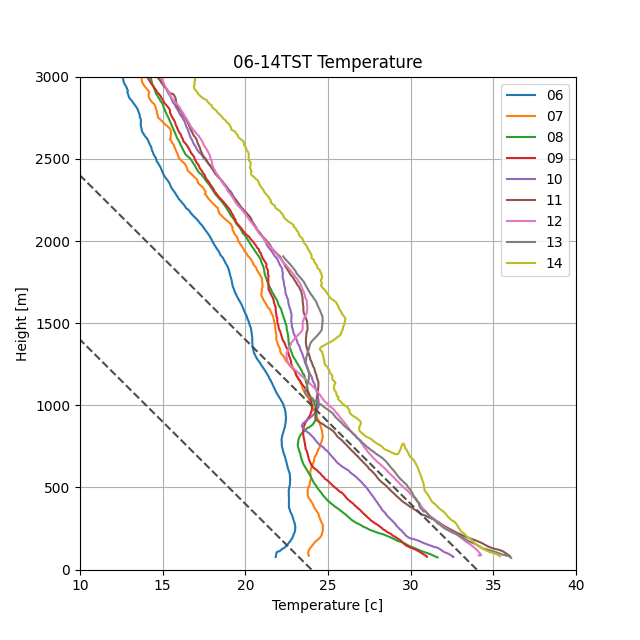
\includegraphics[scale=0.47]{1_a.png}
    %\caption{fig1}
    \end{minipage}%
    }%
    \subfigure[Height - Potential Temp.]{
    \begin{minipage}[t]{0.5\linewidth}
    \centering
    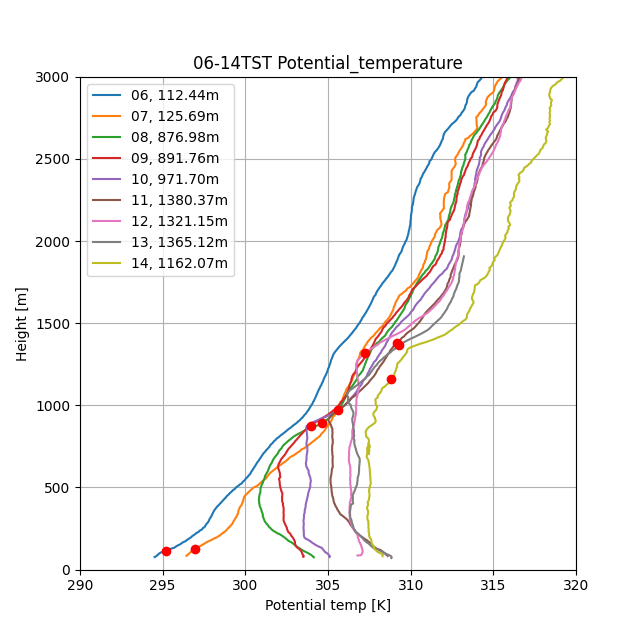
\includegraphics[scale=0.47]{1_b.png}
    %\caption{fig2}
    \end{minipage}%
    }%
\end{figure}


%\newpage

\subsection*{(2)}
\begin{spacing}{2}
    \begin{large}
        \qquad \;如上(a)圖所示, 06 時及07 時氣溫隨高度下降的幅度較小,亦無明顯逆溫層。上午08 時後1000 公尺以下之空氣層其溫度遞減率
        與乾絕熱溫度遞減率相近,表示此大氣層在此期間為中性穩定度。(b)圖則顯示了垂直高度與位溫的關係。紅點標記表示了以$ \theta_{ABL} = \theta_{sfc} + 0.5K $之定義所計算出來之邊
        界層高度。同樣以06、07時為分界,前兩小時計算所得邊界層高度接近,皆約為110至120公尺處,位溫隨高度遞增表示穩定。而08 時後由位溫的垂直分布可以
        看出大氣層有CPBL的特徵,混合層內為均勻混合,且其邊界層高度分布約位於混合層頂部、位溫開始回升處。
    \end{large}
\end{spacing}

\newpage
\thispagestyle{empty}
\hfill {\scshape \large Synoptic Meteorology, Fall 2023 } \hfill {\scshape P2}
\smallskip
\hrule
\bigskip
\section*{2.}

\begin{figure}[!htbp]
    \centering
    \subfigure[Height - Temp.]{
    \begin{minipage}[t]{0.5\linewidth}
    \centering
    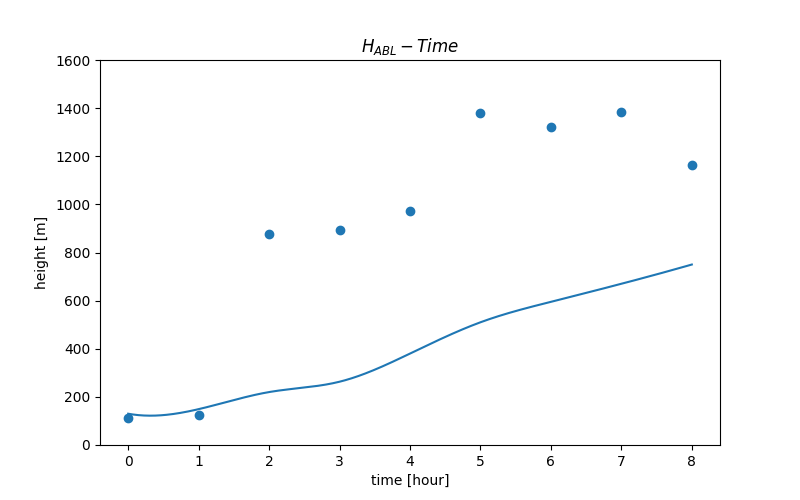
\includegraphics[scale=0.4]{2_1.png}
    %\caption{fig1}
    \end{minipage}%
    }%
    \subfigure[Height - Potential Temp.]{
    \begin{minipage}[t]{0.5\linewidth}
    \centering
    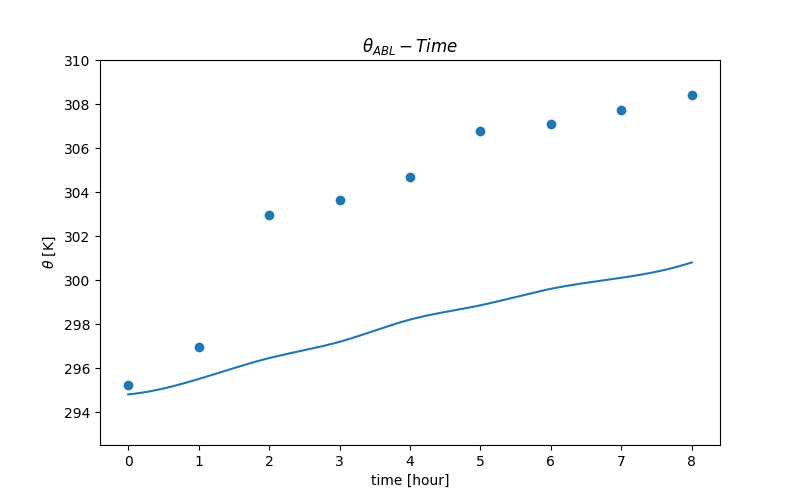
\includegraphics[scale=0.4]{2_2.png}
    %\caption{fig2}
    \end{minipage}%
    }%
\end{figure}
\;\\
\begin{spacing}{2}
    \begin{large}
    \quad由以上兩圖可以發現\;$\theta_{ABL}$及$H_{ABL}$的觀測資料與理論結果皆有一定的差距,理論值皆小於觀測值。其走向符合因Q隨時間增加
    而增加。而理論數值較低的原因可能來自於拿06時的探空資料做計算的這個初始設定。因06時之邊界層較穩定,能使邊界層均勻混合的可感熱在每個時間
    點不成比例。
    \end{large}
\end{spacing}



\end{CJK*}
\end{document}